%\documentclass[journal, onecolumn, letterpaper]{IEEEtran}
%\documentclass[journal,onecolumn]{IEEEtran}
% \documentclass[conference]{IEEEtran}
\documentclass[a4paper, 12pt, onecolumn,singlespacing]{article}

% The preceding line is only needed to identify funding in the first footnote. If that is unneeded, please comment it out.
\usepackage[level]{fmtcount} % equivalent to \usepackage{nth}
% \include{util}
\usepackage[portuguese, brazil, english]{babel}
\usepackage{multirow}
\usepackage{array} % for defining a new column type
\usepackage{varwidth} %for the varwidth minipage environment
\usepackage[super]{nth}
\usepackage{authblk}
\usepackage{cite}
\usepackage{amsmath,amssymb,amsfonts}
\usepackage{ulem}
\usepackage{graphicx}
% \usepackage{subfig}
\usepackage{textcomp}
\usepackage{xcolor}
\usepackage{mathptmx}
\usepackage[T1]{fontenc}
\usepackage{textcomp}
\usepackage{titlesec}
\usepackage{helvet}
\usepackage{gensymb}
\usepackage{setspace} % espacamento entre linhas
\usepackage{pgfplots}
\usepackage{tikz}
\usepackage{subcaption}
\usepackage{minted}
\usepackage[left=2cm, right=2cm, bottom=2cm, top=2cm]{geometry} 
\usepackage{makecell}
\usepackage{pdfpages}


\usepackage{hyperref}
\usepackage{fancyhdr}
\renewcommand{\headrulewidth}{1pt}
\renewcommand{\footrulewidth}{0.5pt}
\fancyhf{} % limpa os cabecalhos e rodapés
\fancyhead[C]{\textit{CURSO DE ENGENHARIA DOS RAIOS - TE981} } % define o cabeçalho personalizado
\fancyfoot[C]{\textit{AUGUSTO MATHIAS ADAMS}}
\pagestyle{fancy} % sem definir esse comando, o cabeçalho personalizado não é exibido

\hypersetup{
	colorlinks=true,
	linkcolor=blue,
	filecolor=magenta,      
	urlcolor=blue,
	pdftitle={ENGENHARIA DOS RAIOS - TE981 - ONE MINUTE PAPER}
}
\renewcommand\theadalign{bc}
\renewcommand\theadfont{\bfseries}
\renewcommand\theadgape{\Gape[4pt]}
\renewcommand\cellgape{\Gape[4pt]}

%dashed line
\usepackage{booktabs, makecell}
\renewcommand\theadfont{\bfseries}
\renewcommand\theadgape{}
\usepackage{arydshln}
\setlength\dashlinedash{0.2pt}
\setlength\dashlinegap{1.5pt}
\setlength\arrayrulewidth{0.3pt}

% padrao 1.5 de espacamento entre linhas
\setstretch{1.5}
\makeatletter
\def\@maketitle{%
	\newpage
	\null
	\vskip 2em%
	\begin{center}%
		\let \footnote \thanks
		{\LARGE \@title \par}%
		\vskip 1.5em%
		{\large
			\lineskip .5em%
			\begin{tabular}[t]{c}%
				\@author
			\end{tabular}\par}%
		%\vskip 1em%
		%{\large \@date}%
	\end{center}%
	\par
	\vskip 1.5em}
\makeatother

\title{\normalsize{ENGENHARIA DOS RAIOS - TE981}\\ \huge{\textbf\textit{{AULA 17 - REPRESENTAÇÃO DO CAMPO ELÉTRICO POR DESCARGAS}}\\}}
\author{\small{AUGUSTO MATHIAS ADAMS}}
\setcounter{Maxaffil}{0}
\renewcommand\Affilfont{\itshape\small}

\begin{document}
	% Seleciona o idioma do documento
	\selectlanguage{brazil}
	
	% título
	\maketitle
	
	\section{Aprendizado da Aula}
	
	\paragraph{Contextualização}
		O sensor Field Mill é um dispositivo essencial na detecção e medição do campo elétrico na atmosfera. Ele consiste em um conjunto de placas condutoras sensíveis ao campo elétrico, dispostas em um arranjo circular ou em formato de moinho. Essas placas são eletricamente isoladas e podem girar livremente em torno de um eixo central.
		
		O princípio de funcionamento do sensor Field Mill baseia-se na interação entre as placas condutoras e o campo elétrico ambiente. Quando um campo elétrico está presente, ocorre uma redistribuição de cargas nas placas do sensor. Isso cria uma diferença de potencial entre as placas, que é medida e registrada por meio de circuitos eletrônicos associados ao sensor.
		
		A rotação das placas é realizada por um motor ou por forças do vento. À medida que as placas giram, diferentes áreas são expostas ao campo elétrico, permitindo a medição em diferentes direções. A taxa de rotação das placas pode variar dependendo da aplicação e das necessidades de amostragem do campo elétrico.
		
		O sensor Field Mill é amplamente utilizado em estudos meteorológicos e de descargas atmosféricas. Ele fornece informações valiosas sobre as características do campo elétrico na atmosfera, como sua intensidade, direção e variabilidade temporal. Esses dados são cruciais para entender os processos elétricos que ocorrem nas tempestades e outras fenômenos atmosféricos, além de contribuir para a previsão e monitoramento de tempestades e descargas elétricas.
		
		É importante ressaltar que o sensor Field Mill é um dos vários tipos de sensores utilizados para medir o campo elétrico atmosférico. Outros métodos de medição, como sensores de carga, antenas e radares, também são empregados para obter uma visão abrangente e precisa das propriedades elétricas da atmosfera. A combinação desses diferentes sensores e técnicas de medição contribui para um melhor entendimento dos fenômenos elétricos na atmosfera e sua relação com o clima e o meio ambiente.
		
		\paragraph{Representação do Campo Elétrico Por Descargas}
		
		Atualmente, não é possível prever com precisão a ocorrência de um raio com base nos valores de campo elétrico medidos pelo Field Mill. Altos valores de campo elétrico não garantem necessariamente que ocorrerá uma descarga, e também não é possível distinguir o comportamento do campo elétrico para descargas entre nuvem e solo ou descargas intra-nuvem.
		
		O desafio está em determinar as circunstâncias em que tais previsões podem ser feitas de forma confiável, minimizando a taxa de alarmes falsos. Estima-se que o campo elétrico próximo ao solo seja proporcional à quantidade de carga elétrica presente.
		
		O campo elétrico total ($E_{total}$) é dado por:
		
		\begin{equation}
			E_{total} = \frac{QH}{2 \pi \epsilon_0 \left(H^2 + D^2\right)^{\frac{3}{2}}}
		\end{equation}
	
		onde $Q$ é o montante de carga elétrica [$C$] no centro onde o raio se origina, $H$ é a altura [$m$] do centro de cargas elétricas na nuvem, $\epsilon_0$é a permissividade elétrica [$F/m$] e $E_{total}$ é a média do campo elétrico abaixo da tempestade [$V/m$].
		
		Do exemplo dado em sala, a distância estimada é dada por:
		
		\begin{equation}
			D = \sqrt{\left[\frac{QH}{2 \pi \epsilon_0 E_{total}}\right]^{2/3} -H^2}
		\end{equation}
	
		Outra expressão também é usada para estimar a distância de uma descarga atmosférica a partir das informações de um sistema de monitoramento. Usando a latitude e a longitude reportada por uma rede de monitoramento, cada \textit{stroke} pode ter a distância estimada (em $km$) até um ponto de localização pretendido, através da equação:
		
		\begin{equation}
			D = 2 R_e arcsen\left(\sqrt{sen^2\left(\frac{\theta_0-\theta_e}{2}\right) + cos(\theta_0) cos (\theta_e) sen^2\left(\frac{\phi_0 - \phi_e}{2}\right)}\right)
		\end{equation}
	
		onde $R_e = 6378 km$ é o raio médio da Terra, assumindo uma forma esférica. $\theta_0$ é a latitude do ponto de localização (em graus), $\phi_e$ é a latitude do raio predito pela rede de monitoramento, $\theta_e$ é a longitude do ponto pretendido (em graus), e $\phi_e$ é a longitude do raio estimado pela rede de monitoramento, também em graus.
		Com esta equação é possível estimar o pico de corrente da descarga atmosférica $I$, medida com um campo elétrico $E$, e com distância estimada por uma rede de monitoramento $D$, usando a equação de regressão derivada por Rakov et. al. (1992):
		
		\begin{equation}
			I = 1,5 - 0.037 DE
		\end{equation}
	
		onde, $I$ é a corrente elétrica em $kA$ e considerado negativo, $E$, é positivo e em $V/m$, e $D$ é a distância estimada em $km$. Segundo estudos esta expressão apresenta uma diferença percentual entre o pico de corrente teórico (calculado pela equação anterior) e o pico de corrente estimado por uma rede de monitoramento de descargas atmosféricas, e que
		pode ser dada como:
		
		\begin{equation}
			\Delta I\% = \frac{\left|I_{estimado}\right| - \left|I_{teorico}\right|}{\left|I_{estimado}\right|} \times 100
		\end{equation}
	
		\paragraph{Perfil de Campo Elétrico}
		
		Os estudos realizados por Moore et al. (1959) e Malan (1963) sugerem que durante os estágios iniciais e de maturidade de uma nuvem de tempestade, ocorre um acúmulo de cargas elétricas positivas em sua base inferior, próxima à superfície terrestre. Essa eletrificação inicial pode ser identificada nas medições do perfil do campo elétrico local pela mudança de polaridade na intensidade do campo mensurado.
		
		De acordo com os estudos apresentados por Golde (1977), os estágios de uma tempestade podem ser identificados pela observação do perfil do campo elétrico local dessa tempestade.
		
		À medida que o evento avança, a nuvem de tempestade atinge o estágio de maturidade, e íons positivos começam a descer juntamente com a precipitação, resultando no surgimento de picos secundários no gradiente de potencial, conhecidos como comportamentos duplos do potencial em curtos intervalos de tempo, associados à direção da precipitação.
		
		A fase de dissipação da tempestade é caracterizada pelo gradiente de potencial, que indica o fim do processo de oscilação das cargas dentro da nuvem. Durante essa fase, é observada uma variação prolongada do gradiente, e o estágio seguinte corresponde à dissipação completa da tempestade.
		
		Ao analisar o perfil do campo elétrico de um raio, é possível estudar a forma de onda do campo elétrico (E) e a forma de onda do campo magnético (B).
		
		\subparagraph{Processos J e K}
		Os processos J e K são fenômenos elétricos que ocorrem durante descargas atmosféricas, como raios. Eles estão relacionados às variações do campo elétrico entre as diferentes etapas da descarga.
		
		O processo J refere-se a uma mudança relativamente estável no campo elétrico que ocorre durante o intervalo de tempo entre as descargas principais, conhecidas como \textit{``return strokes''}. O campo elétrico durante o processo J pode ter uma mudança positiva ou negativa, e é geralmente menor do que a mudança de campo devido à corrente contínua da descarga principal. Diferente da descarga principal, o processo J não está associado a um canal luminoso entre a nuvem e o solo.
		
		Por outro lado, o processo K envolve variações rápidas e relativamente pequenas no campo elétrico que ocorrem entre as descargas principais, em intervalos de tempo de 2 a 20 milissegundos. Essas variações, conhecidas como \textit{``K-changes''}, são superpostas à mudança geral do campo elétrico associado ao processo J. O processo K é frequentemente interpretado como a ocorrência de pequenas descargas ou \textit{``streamers''} que se movem dentro da nuvem, fornecendo uma contribuição para as variações do campo elétrico entre as descargas principais.
		
		A interpretação exata dos processos J e K e seu papel na dinâmica das descargas atmosféricas ainda é objeto de estudo e debate entre os pesquisadores. Diferentes teorias e observações têm sido propostas para explicar esses processos, e pesquisas adicionais são necessárias para um melhor entendimento de sua natureza e mecanismos subjacentes.

		A figura \ref{lightning_process} mostra as etapas de um processo de descarga, visto no espectro óptico:
		
		\begin{figure}[h]
			\centering
			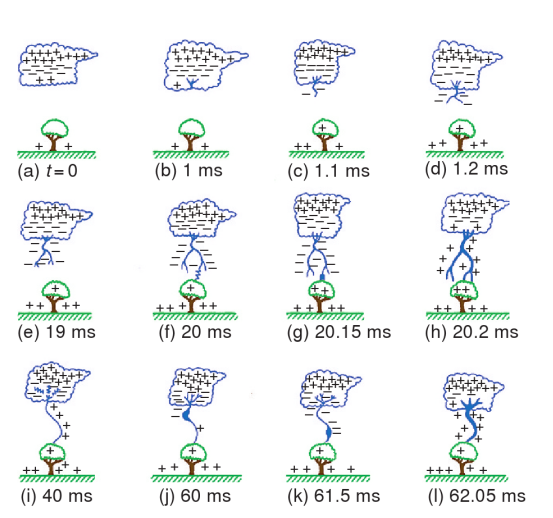
\includegraphics[width=0.6\textwidth]{imagens/lightning_process.png}
			\caption{Esquemático para ilustrar alguns dos processos que levam a um raio no solo que carrega o solo negativamente. (a) Distribuição de carga na nuvem, (b) Quebra Inicial, (c-e) Líder Escalonado, (f) Processo de conexão, (g e h) Primeira descarga de retorno, (i) Processos K e J, (j e k) Líder em dardo e (1) Segunda descarga de retorno. [Adaptado de M. Uman, The Lightning Discharge, Academic Press, Inc., Nova York, 1987, p. 12, Direitos autorais 1987, com permissão da Elsevier.]}
			\label{lightning_process}
		\end{figure}
		
		Etapas explicadas: 
		
		\begin{itemize}
			\item  \textbf{\textit{ (a) Distribuição de carga na nuvem:} }Nesta etapa, a nuvem contém uma separação de cargas positivas e negativas. Tipicamente, a parte inferior da nuvem está carregada negativamente, enquanto a parte superior está carregada positivamente.
			
			\item \textbf{\textit{(b) Quebra Inicial:}} Uma região da nuvem próxima ao solo experimenta um campo elétrico forte, o que leva à iniciação de uma pré-quebra. Esse processo envolve o desenvolvimento de canais de ionização que conectam a nuvem ao solo.
			
			\item \textbf{\textit{(c-e) Líder escalonado:}} O líder escalonado é uma série de canais luminosos e escalonados que se propagam de cima para baixo a partir da nuvem em direção ao solo. Consiste em uma série de descargas rápidas ou degraus, cada uma durando microssegundos. O líder escalonado busca um caminho de menor resistência em direção ao solo, ramificando-se e se estendendo de maneira irregular.
			
			\item \textbf{\textit{(f) Processo de conexão:}} Quando o líder escalonado se aproxima do solo, estabelece-se uma conexão entre ele e um líder invisível em movimento ascendente chamado líder em dardo. Essa conexão é conhecida como processo de conexão.
			
			\item \textbf{\textit{(g e h) Primeira descarga de retorno:}} A primeira descarga de retorno é o canal luminoso principal que transporta a maior parte da corrente do raio do solo para cima. Ocorre após o processo de conexão e se desloca rapidamente ao longo do caminho estabelecido pelo líder escalonado. A primeira descarga de retorno é a parte brilhante e visível do raio.
			
			\item \textbf{\textit{(i) Processos K e J:}} Após a primeira descarga de retorno, pode haver variações no campo elétrico conhecidas como processos K e J. O processo K refere-se a flutuações menores e rápidas no campo elétrico, enquanto o processo J representa uma mudança mais lenta e gradual no campo elétrico.
			
			\item \textbf{\textit{(j e k) Líder \textit{``dart''}:}} Após a primeira descarga de retorno, um novo líder chamado líder \textit{``dart''} se propaga de cima para baixo a partir da nuvem em direção ao solo. O líder \textit{``dart''} segue um caminho mais direto e menos ramificado em comparação com o líder escalonado.
			
			\item \textbf{\textit{(1) Segunda descarga de retorno: }}O líder \textit{``dart''} atinge o solo, e ocorre uma segunda descarga de retorno, semelhante à primeira. Essa segunda descarga de retorno geralmente é menos intensa do que a primeira.
			
		\end{itemize}
		
		Esses processos descrevem a sequência geral de eventos que levam a um flash no solo que carrega o solo negativamente. Referências visuais ou esquemas podem fornecer uma representação mais detalhada e precisa desses processos.
		
		\paragraph{Componente M} Uma evidência óptica rara em alta velocidade do mecanismo da componente M de onda-guiada, adaptada de Jiang et al. (2014), é mostrada na Figura \ref{Component_M_explained}. Nos quadros (a) e (b), um líder de recuo (parte negativa) se desenvolve ao longo de um ramo decadente de um líder positivo ascendente iniciado a partir de uma torre de 112 m. Havia pelo menos seis ramos de líder positivo ascendente, a maioria dos quais são muito fracos para serem vistos na reprodução. Um canal portador de corrente conectado à torre é claramente visível nos seis quadros. No quadro (c), o líder de recuo se conecta ao canal aterrado, a 350 m acima do topo da torre (R. Jiang, comunicação pessoal, 8 de janeiro de 2018), e lança uma onda M incidente em direção à ponta da torre. Em algum momento entre os quadros (c) e (d), a onda M incidente chega à ponta da torre e produz uma onda M refletida no solo, o que causa o brilho e a extensão da parte superior do canal do líder de recuo (veja os quadros e e f). (Também pode haver reflexão parcial a partir do ponto de junção que não é considerado parte da componente M.) Vale ressaltar que o evento mostrado na Figura \ref{Component_M_explained} é um pulso de ICC, que pode ser um evento de modo misto (Zhou et al., 2015), uma vez que a altura do ponto de junção (350 m) acima do topo da torre é inferior a 1 km. No entanto, este evento ilustra essencialmente o mecanismo da componente M.
		
		\begin{figure}[!h]
			\centering
			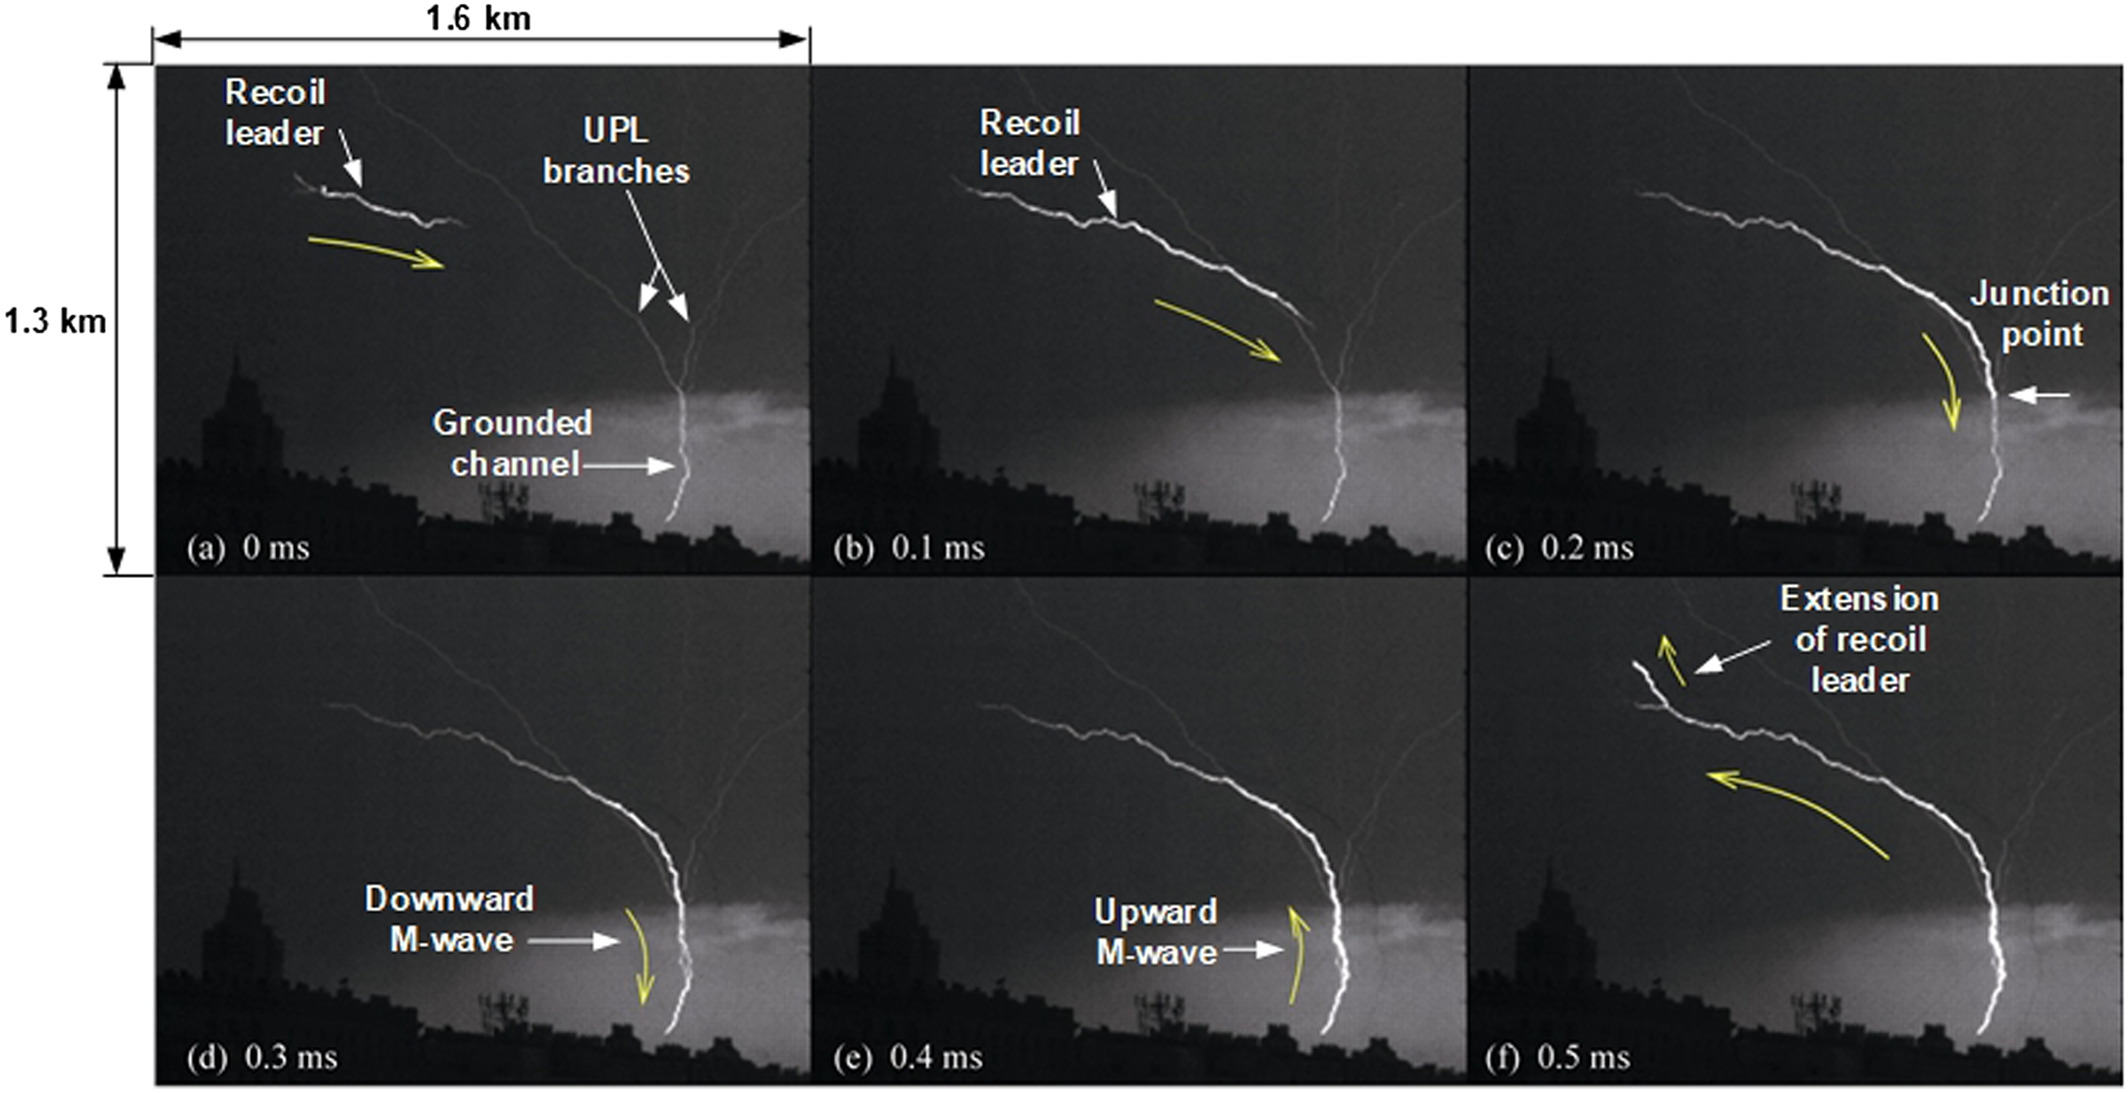
\includegraphics[width=\textwidth]{imagens/processo_componente_m.jpg}
			\caption{Evidência óptica do mecanismo da componente M de onda-guiada exibido por um pulso inicial de corrente contínua ascendente de um relâmpago negativo iniciado a partir de uma torre de 112 m. Mostradas nas figuras (a) a (f) estão seis quadros consecutivos separados por 100 $\mu s$, nos quais é possível observar um líder de recuo em um ramo decadente de um líder positivo ascendente que faz conexão com o canal aterrado e portador de corrente e inicia uma onda M descendente ao longo desse canal, do ponto de junção à ponta da torre, seguida por uma onda M ascendente refletida no solo que refaz e estende o canal do líder de recuo. Adaptado de Jiang et al. (2014)}
			\label{Component_M_explained}
		\end{figure}
		
		\section{Temas Impactantes, dúvidas e questionamentos}
		
		Nada que os livros e artigos não possam sanar. Depois de fazer o trabalho sobre descargas negativas descendentes nuvem-solo, também não é surpresa alguma um tema semelhante.
		
\end{document}